\documentclass[12pt,a4paper]{article}
\usepackage[utf8]{inputenc}
\usepackage[russian]{babel}
\usepackage{graphicx}
\usepackage{listings}
\begin{document}
\section{Постановка задачи}
Результатом выполнения лабораторной работы должен быть файл содержащий следующие основные части:
\begin{enumerate}
    \item Описание предметной области.
    \item Инфологическая (Концептуальная) модель базы данных для выбранной предметной области.
    \item Логическая модель базы данных для выбранной предметной области.
\end{enumerate}
\section{Построение концептуальной модели базы данных}
В качестве предметной области для примера выберем объекты киноиндустрии.\par
Основные сущности это произведение киноиндустрии(фильм, сериал и т.д.) и деятель киноиндустрии (актер, режиссер, директор).
В качестве основных атрибутов произведения можем выделить:
\begin{enumerate}
    \item \textbf{titleID} - буквенно-цифровой уникальный идентификатор заголовка.
    \item \textbf{titleType} – формат заголовка (например, фильм, короткометражка, сериал, твизод, видео и т.д.).
    \item \textbf{primaryTitle} – более популярное название / название, используемое создателями фильма в рекламных материалах на момент выпуска.
    \item \textbf{originalTitle} - оригинальное название, на языке оригинала.
    \item \textbf{isAdult} - запрещено к просмотру лицам не достигшим совершеннолетия.
    \item \textbf{startYear} – год выпуска.
    \item \textbf{runtimeMinutes} – длительность произведения в минутах.
    \item \textbf{posterURL} - URL постера.
    \item \textbf{plot} - сюжет.
\end{enumerate} \par
Введем cущностью рейтинг произведения со следующими атрибутами:
\begin{enumerate}
    \item \textbf{ratingID} - буквенно-цифровой уникальный идентификатор рейтинга 
    \item \textbf{averageRating} - средний рейтинг произведения.
    \item \textbf{numVotes} - количество голосов которые получил фильм.
    \item \textbf{ratingType} - тип рейтинга (IMDB, Metacritic и т.д.)
\end{enumerate} \par
Каждое произведение имеет 1 ко многим связь с сущностью рейтинг. Так как у одного произведения может быть множество рейтингов. \par
Каждое произведение имеет 1 ко многим связь с сущностью жанр со следующими атрибутами:
\begin{enumerate}
    \item \textbf{genreID} - буквенно-цифровой уникальный идентификатор жанра
    \item \textbf{genreType} - тип жанра (драма, комедия и т.д.)
\end{enumerate} \par
Если произведение киноинудстрии является сериалом имеет смысл ввести сущность эпизод. Имеющую следующие атрибуты:
\begin{enumerate}
    \item \textbf{titleID} - идентификатор серии сериала.
    \item \textbf{parentTitleID} - буквенно-цифровой идентификатор сериала к которому относится эпизод.
    \item \textbf{seasonNumber} - номер сезона.
    \item \textbf{episodeNumber} - номер серии в сезоне.
\end{enumerate} \par
Связь произведения с сущностью эпизод будет 1 ко многим. Так как у одного сериала может быть множество эпизодов. \par
Перейдем к сущности деятеля киноидустрии. В качестве основых атрибутов можем выделить:
\begin{enumerate}
    \item \textbf{nameID} - буквенно-цифровой уникальный идентификатор деятеля киноинудстрии.
    \item \textbf{primaryName} - имя, под которым деятель упоминается в произведениях.
    \item \textbf{birthYear} - дата рождения.
    \item \textbf{deathYear} - дата смерти.
\end{enumerate} \par
У каждого деятеля киноидустрии есть список профессий (режиссер, директор, актер и т.д.) вынесем это в отдельную сущность профессия имеющую атрибуты:
\begin{enumerate}
    \item \textbf{professionID} - буквенно-цифровой уникальный идентификатор профессии.
    \item \textbf{jobType} - тип профессии (режиссер, директор, актер и т.д.).  
\end{enumerate} \par
Связь между деятелем киноидустрии и профессией будет один ко многим. Так как у одного деятеля киноиндустрии может быть множество профессий. 
И наоборот может быть множество деятелей киноиндустрии с одинаковой профессией. \par
Для связи между произведением киноидустрии, деятелем киноидустрии и профессией введем дополнительную сущность участник съемочной группы. \par
Связь между произведением киноиндустрии и участником съемочной группы будет 1 ко многим, 
так как у произведения киноиндустрии может быть множество участников съемочной группы. \par
Связь между деятелем киноиндустрии и участником съемочной группы будет 1 ко многим, 
так как деятель киноиндустрии мог принимать участние в нескольких произведениях. \par
Связь между профессией и участником съемочной группы будет 1 ко многим, 
так как одну и ту же должность занимали множество участников съемочной группы. \par
\begin{figure}[ht]
    \centering
    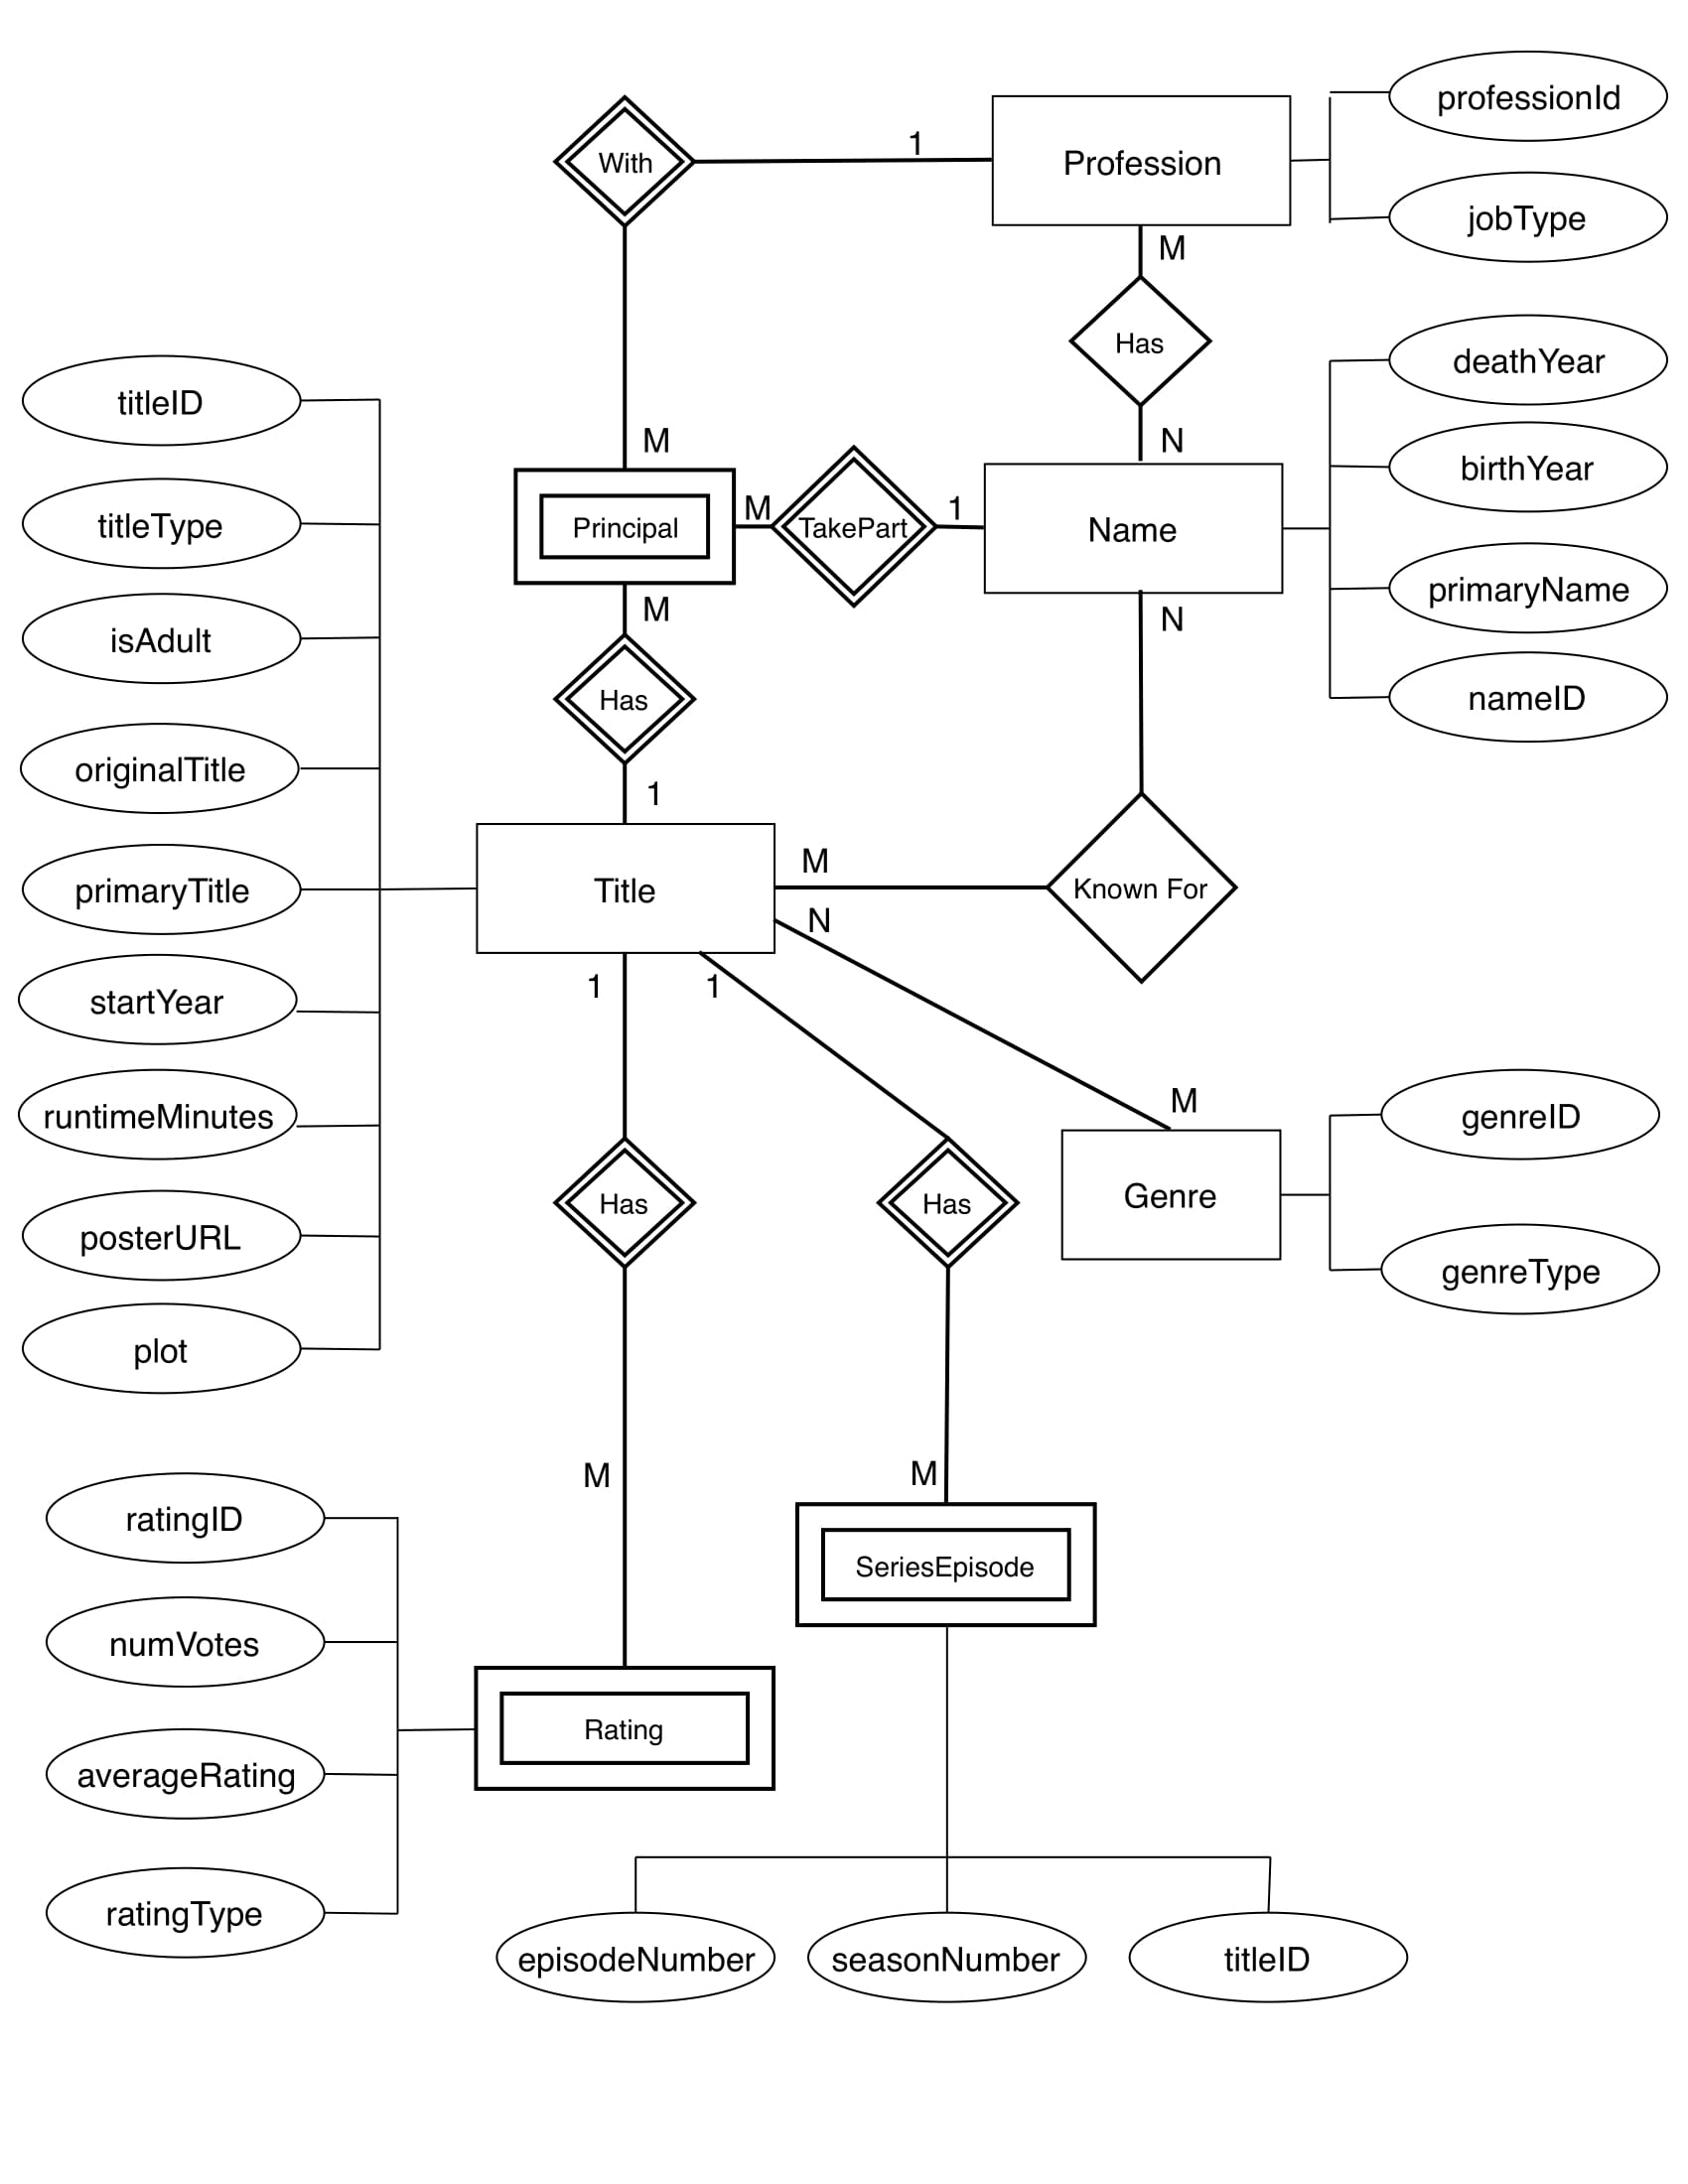
\includegraphics[width=\linewidth]{images/Lab1/conceptual_model.jpg}
    \caption{Conceptual model}
    \label{fig:Conceptual model}
\end{figure}
\section{Логическая модель базы данных}
При построение логичекой модели данных связи многие ко многим реализуются при помощи промежуточной(связывающей) таблицы. \par
Для разрещения связей многие ко многим между сущностями произведение киноиндустрии и участник съемочной группы введем промежуточную таблицу KnownForTitle. \par
Для разрешение связей многие ко многим между профессией и деятелем киноидустрии введем промежуточную таблицу NameProfessions. \par
\begin{figure}[ht]
    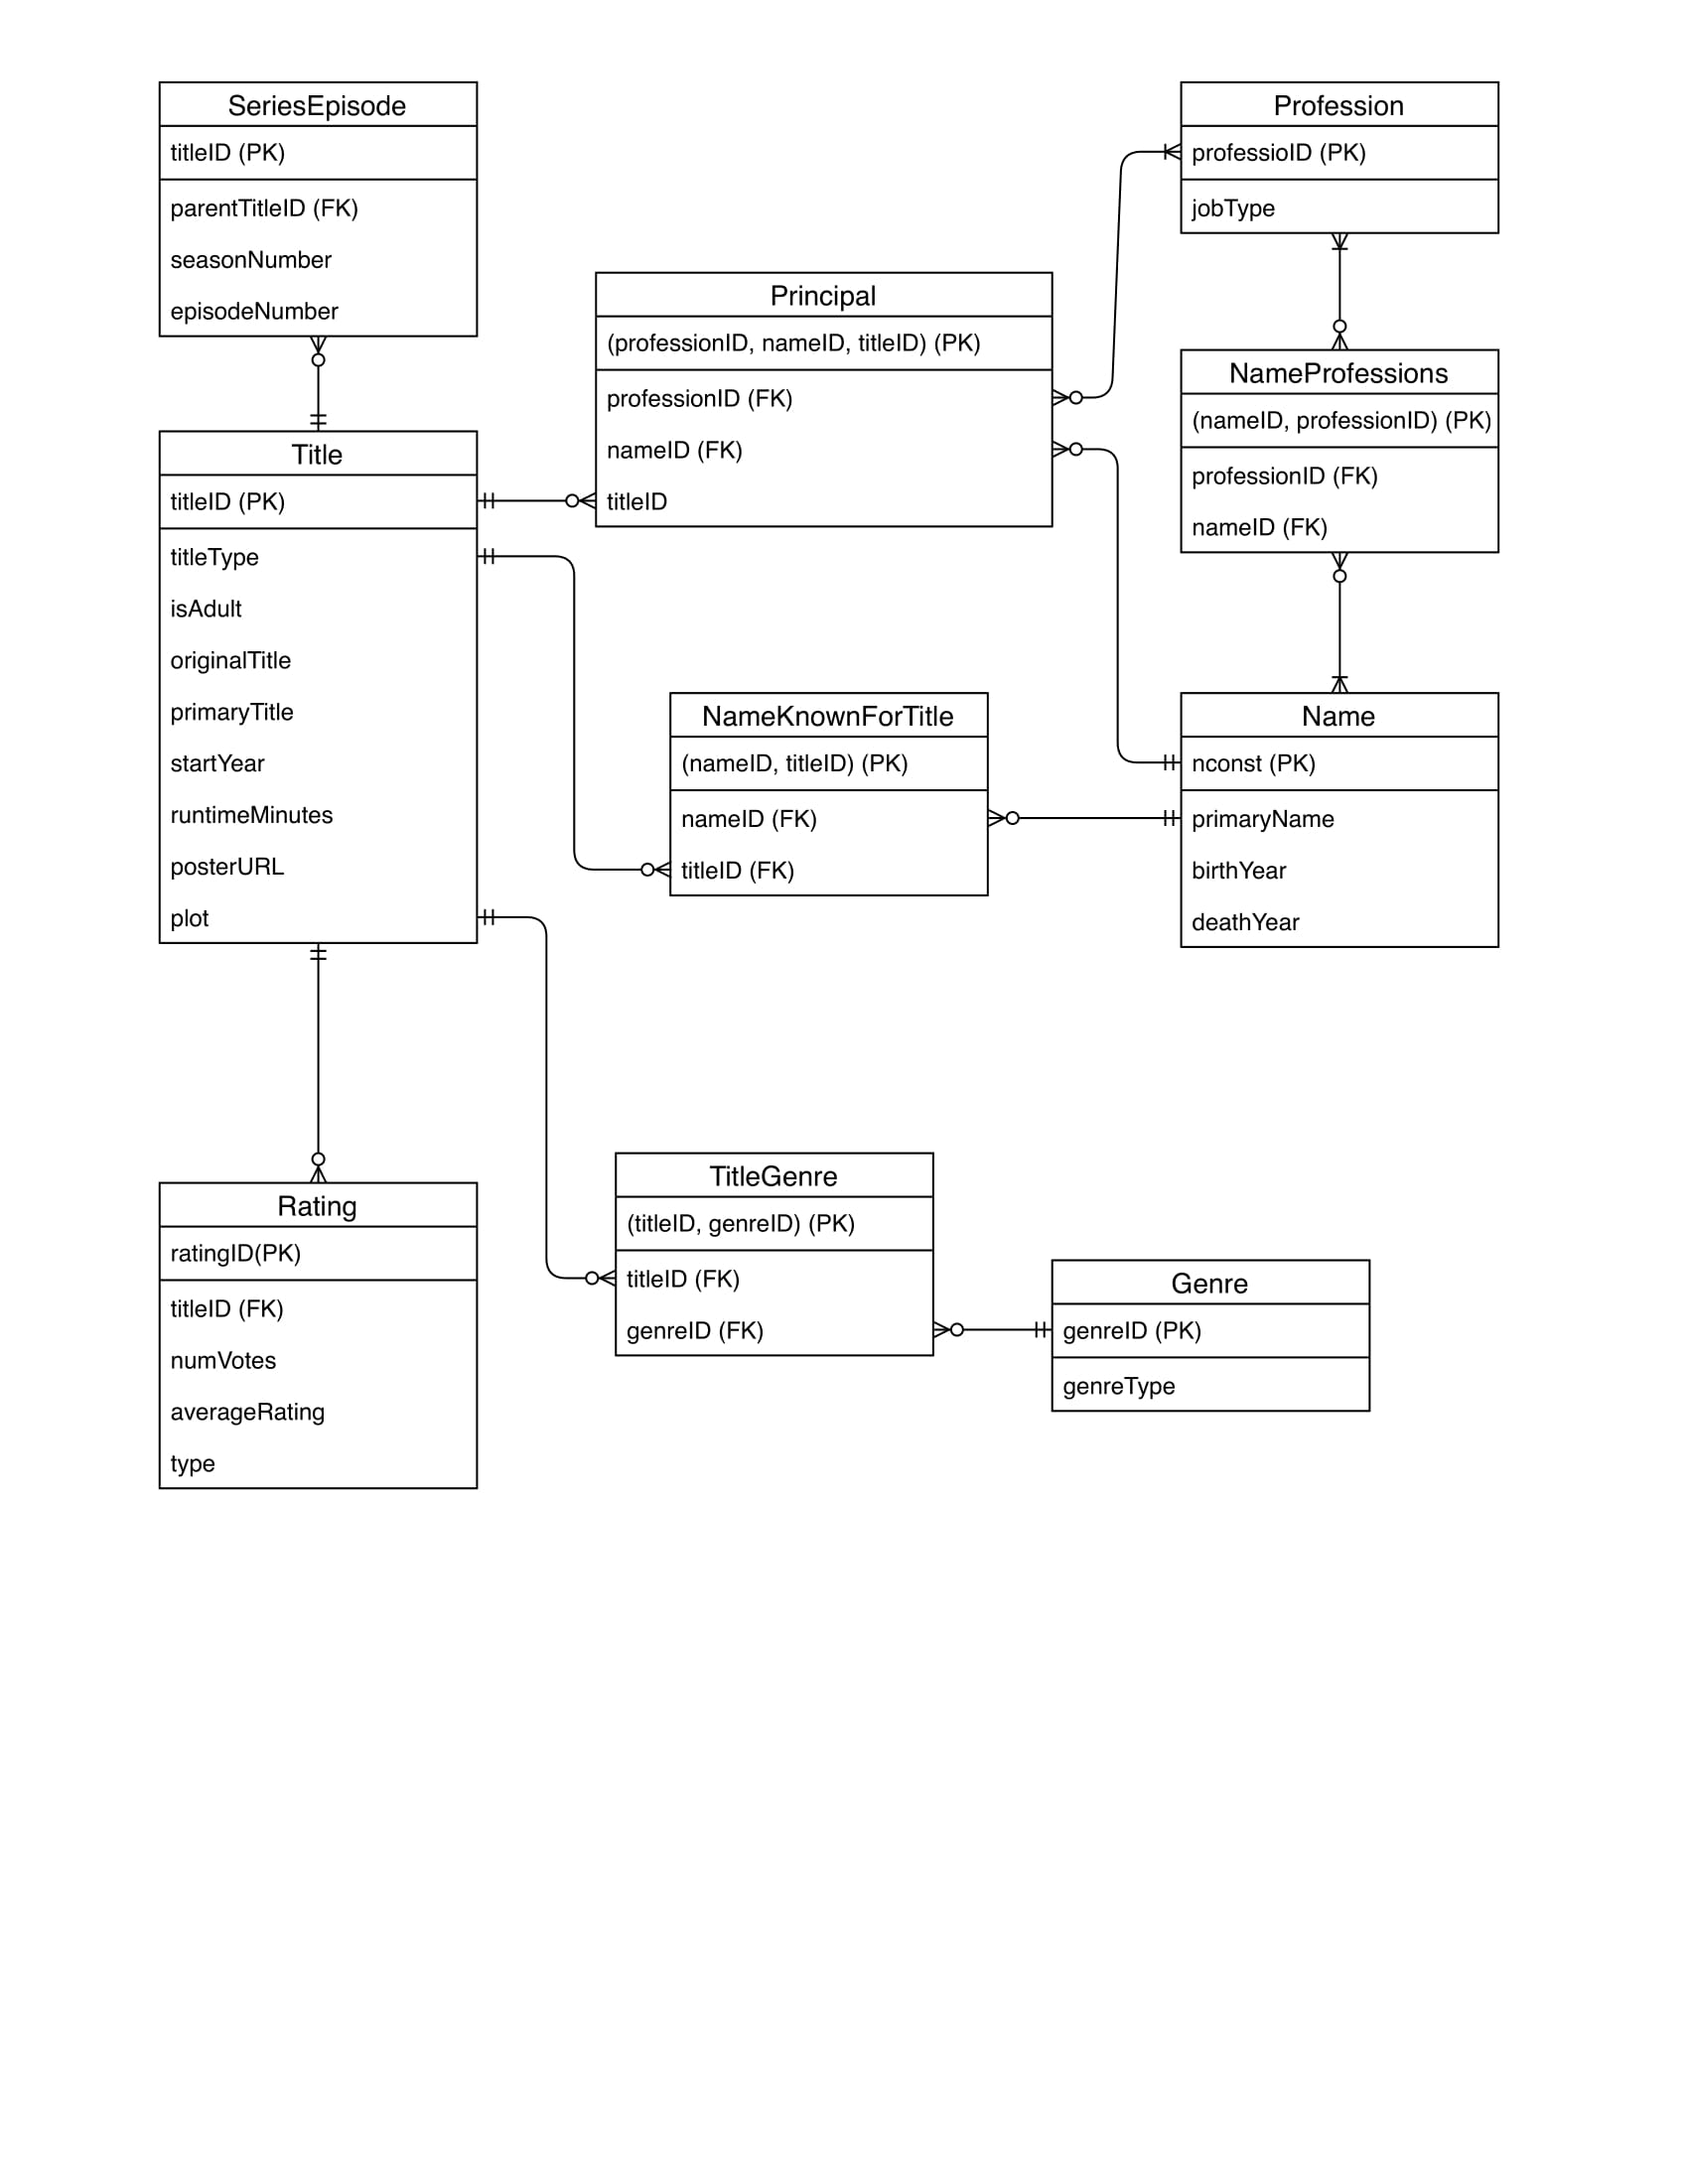
\includegraphics[width=\linewidth]{images/Lab1/logical_model.jpg}
    \caption{Logical model}
    \label{fig:Logical model}
\end{figure}
\section{Используемые источники}
\begin{enumerate}
    \item https://habr.com/ru/post/254773/ (Статья про нормализацию)
    \item https://www.intuit.ru/studies/courses/1095/191/lecture/4983?page=5 (Промежуточная таблица для связи многие ко многим)
\end{enumerate}
\end{document}